Дискретизации подлежат уравнение Рейнольдса (при полном заполнении зазора) и его обобщение JFO~\eqref{eq:jfo_conservation}. В обоих случаях используется консервативная (потоковая) форма записи: для каждой ячейки формулируется баланс потоков через её грани. Такой подход обеспечивает сохранение массы на дискретном уровне и является удобной основой для реализации JFO-условий в кавитационной зоне.

Расчётная область покрывается прямоугольной равномерной сеткой с узлами~$(i,\,j)$ и шагами~$\Delta x_1$,~$\Delta x_2$ (формула~\eqref{eq:jfo_grid} в главе~2). Потоки вычисляются на гранях ячеек: $i \pm 1/2$ по~$x_1$ и $j \pm 1/2$ по~$x_2$. Граничные условия на сетке реализуются в соответствии с разделом~3.1.

Консервативный баланс массы на ячейке~$(i,\,j)$ записывается в виде
\begin{equation}\label{eq:discrete_balance}
  \frac{(\vartheta h)_{i,j}^{n+1} - (\vartheta h)_{i,j}^{n}}{\Delta t}
  + \frac{F_{i+\frac{1}{2},j} - F_{i-\frac{1}{2},j}}{\Delta x_1}
  + \frac{G_{i,j+\frac{1}{2}} - G_{i,j-\frac{1}{2}}}{\Delta x_2}
  = 0,
\end{equation}
\begin{conditions}
$F = F_P + F_C$ -- суммарный поток через грань по~$x_1$ (напорный и переносной);\\
$G = G_P + G_C$ -- аналогичный поток по~$x_2$.
\end{conditions}
При полном заполнении ($\vartheta = 1$) уравнение~\eqref{eq:discrete_balance} сводится к классической дискретизации уравнения Рейнольдса. В стационарной постановке член по времени опускается.

\textit{Напорный (пуазейлевский) поток.}
Коэффициент проводимости определяется как
\[
  K = \frac{h^3}{12\mu}.
\]

Потоки на гранях аппроксимируются центральными разностями:
\begin{equation}\label{eq:flux_poiseuille}
\begin{split}
  &F_{P,\,i+\frac{1}{2},j} = -K_{i+\frac{1}{2},j}\,
    \frac{p_{i+1,j} - p_{i,j}}{\Delta x_1}, \\
  &G_{P,\,i,j+\frac{1}{2}} = -K_{i,j+\frac{1}{2}}\,
    \frac{p_{i,j+1} - p_{i,j}}{\Delta x_2}.
\end{split}
\end{equation}

Коэффициент~$K$ на грани вычисляется усреднением значений в соседних узлах (арифметическое или гармоническое усреднение); при достаточно мелкой сетке различия между арифметическим и гармоническим усреднением, как правило, малы.

\textit{Переносной (куэттовский) поток.}
Для уравнения JFO переносной поток записывается в виде
\begin{equation}\label{eq:flux_couette}
\begin{split}
  &F_{C,\,i+\frac{1}{2},j} = \frac{\vartheta_{\mathrm{up}}\,
    h_{i+\frac{1}{2},j}}{2}\,U_1, \\
  &G_{C,\,i,j+\frac{1}{2}} = \frac{\vartheta_{\mathrm{up}}\,
    h_{i,j+\frac{1}{2}}}{2}\,U_2,
\end{split}
\end{equation}

Значение $\vartheta_{\mathrm{up}}$ выбирается из наветренного узла: при $U_1 \geq 0$ берут $\vartheta_{\mathrm{up}} = \vartheta_{i,j}$, иначе $\vartheta_{\mathrm{up}} = \vartheta_{i+1,j}$; аналогично по~$x_2$: при $U_2 \geq 0$ берут $\vartheta_{\mathrm{up}} = \vartheta_{i,j}$, иначе $\vartheta_{\mathrm{up}} = \vartheta_{i,j+1}$. При полном заполнении ($\vartheta = 1$) множитель~$\vartheta_{\mathrm{up}}$ обращается в единицу. Толщина~$h$ на грани вычисляется арифметическим усреднением. Схема расчётной ячейки с указанием потоков на гранях показана на рисунке~\ref{fig:cell_fluxes}.

\begin{figure}[!ht]
\centering
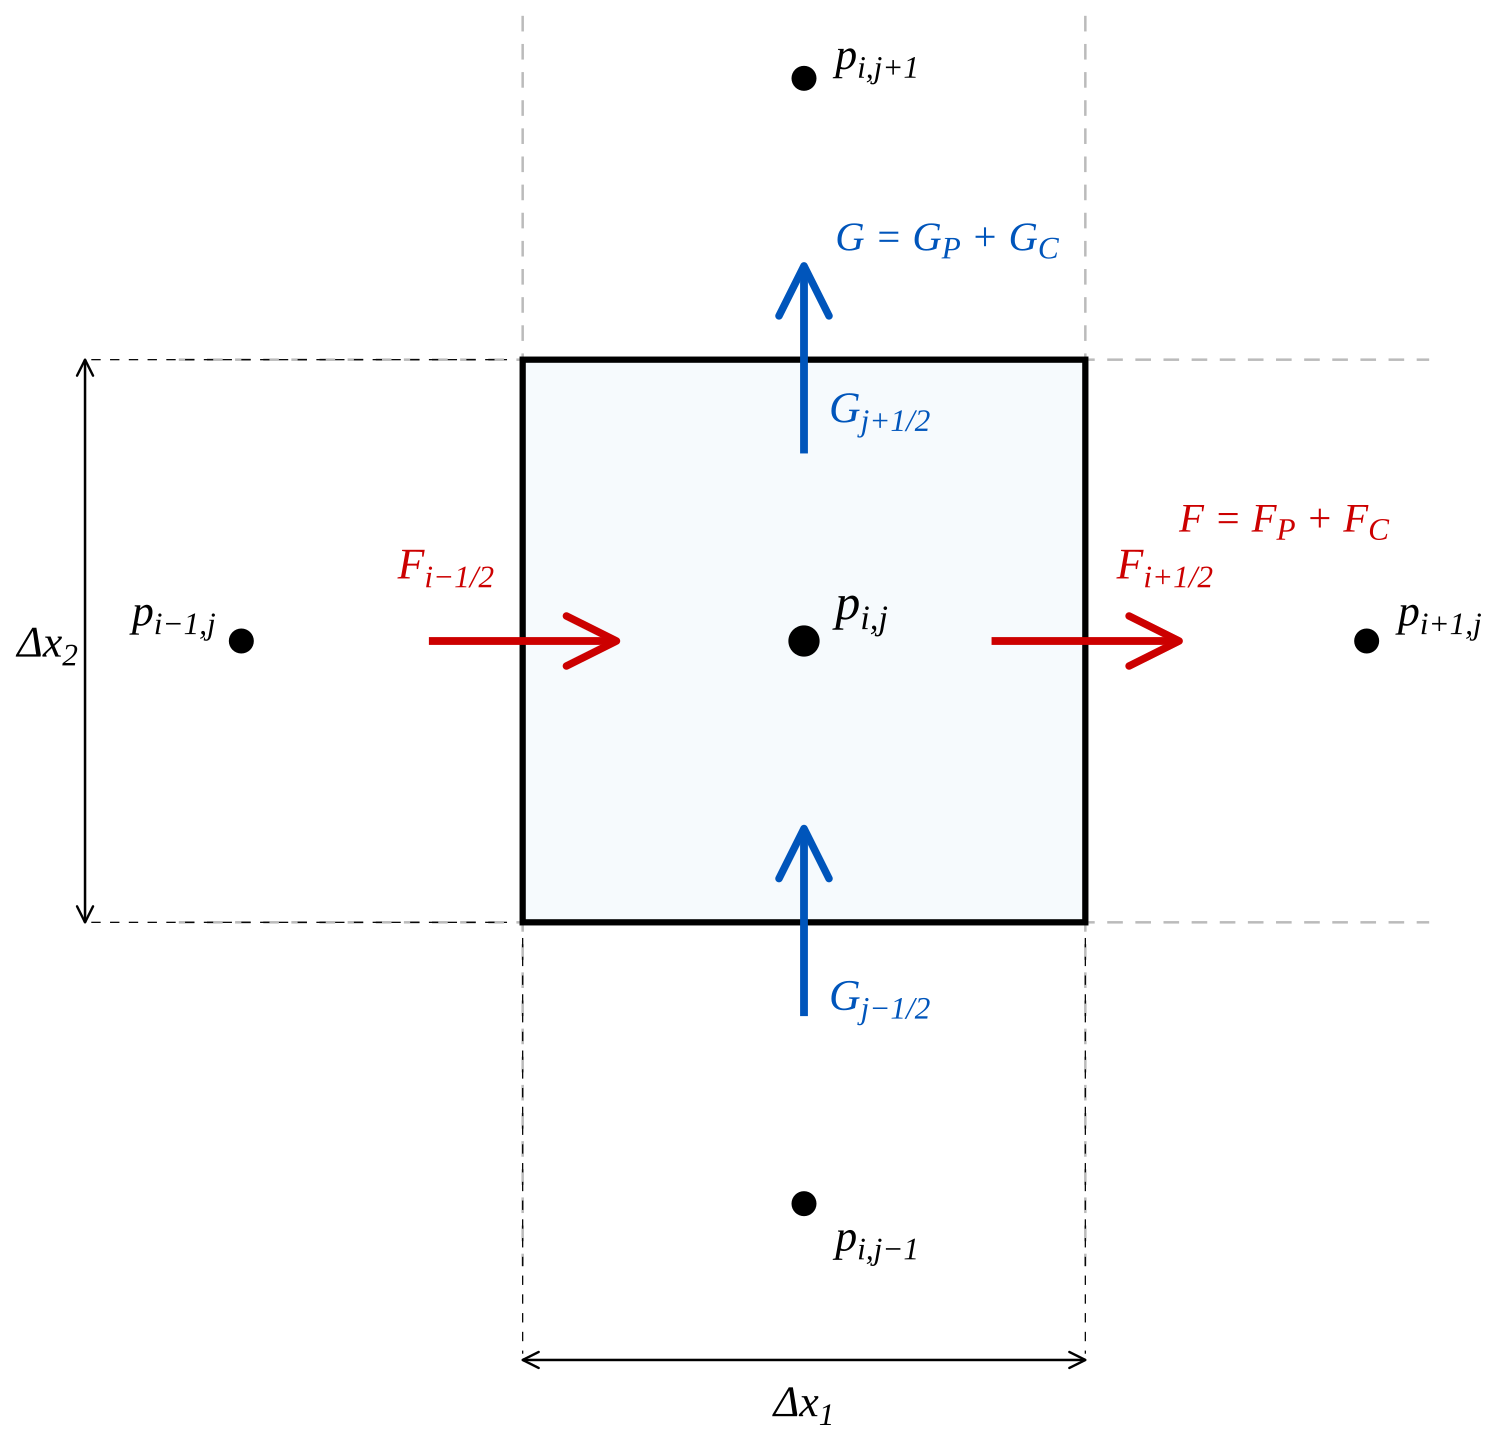
\includegraphics[width=\textwidth,height=0.9\textheight,keepaspectratio]{figures/ch03/fig_3_1.png}
\caption{Схема расчётной ячейки и потоков на гранях}
\label{fig:cell_fluxes}
\end{figure}

\FloatBarrier

\textit{5-точечный шаблон для давления.}
Подстановка потоков в баланс~\eqref{eq:discrete_balance} при $\vartheta = 1$ (стационарный случай) приводит к линейной системе вида
\begin{equation}\label{eq:5point_stencil}
  a_P\,p_{i,j} = a_E\,p_{i+1,j} + a_W\,p_{i-1,j}
    + a_N\,p_{i,j+1} + a_S\,p_{i,j-1} + b_{i,j},
\end{equation}
\begin{conditions}
$a_E$,~$a_W$,~$a_N$,~$a_S$ -- коэффициенты, определяемые проводимостями~$K$ на соответствующих гранях;\\
$a_P = a_E + a_W + a_N + a_S$ -- диагональный коэффициент;\\
$b_{i,j}$ -- правая часть, содержащая вклад куэттовского потока (и, при нестационарности, члена по времени).
\end{conditions}
Система~\eqref{eq:5point_stencil} решается итерационно; выбор решателя описан в разделе~3.3. В нестационарной постановке временной член в~\eqref{eq:discrete_balance} приводит к модификации диагонального коэффициента и правой части разностного уравнения.

В модели JFO давление в кавитационных узлах фиксируется на уровне $p_{\mathrm{cav}}$, поэтому $\nabla p = 0$ и напорные потоки в кавитационной зоне отсутствуют. Обновление активного множества и вычисление~$\vartheta$ в кавитации описаны в разделе~3.5.

Центральные разности для напорного потока обеспечивают второй порядок аппроксимации. Upwind-схема для переноса~$\vartheta$ имеет первый порядок, однако гарантирует устойчивость при доминировании конвективного переноса.

\textit{Порядок аппроксимации и влияние сетки.}
Центральные разности для напорного
потока~\eqref{eq:flux_poiseuille} обеспечивают второй порядок
аппроксимации по $\Delta x_1$, $\Delta x_2$ в узлах, где
зазор $h$ гладко изменяется. В области детерминированных
микроструктур поверхности зазор имеет резкие перепады
на границах элементов рельефа: на переднем склоне лунки $h$
возрастает, на заднем убывает на масштабе нескольких ячеек
сетки. В таких зонах локальный порядок аппроксимации снижается
до первого. Практическое следствие: для корректного
воспроизведения гидродинамического эффекта отдельного элемента
микрорельефа требуется не менее 8--10 узлов на один элемент
вдоль каждого направления. При недостаточном разрешении
коэффициент проводимости~$K_{i+1/2,\,j} =
h_{i+1/2,\,j}^3/(12\mu)$ на грани между «лункой»
и «площадкой» усредняется избыточно, что занижает контраст
потоков и уменьшает расчётный гидродинамический эффект.

\textit{Особенности схемы для цилиндрических координат.}
Для упорного подшипника расчётная область задаётся
в цилиндрических координатах $(r,\,\theta)$. Уравнение
Рейнольдса в этих координатах содержит дополнительные
множители $r$ (перед радиальным потоком) и $1/r$ (перед
угловым): характерные коэффициенты проводимости принимают вид
$K_{r} = r\,h^3/(12\mu)$ и $K_\theta = h^3/(12\mu\,r)$.
В консервативной форме~\eqref{eq:discrete_balance} это
приводит к тому, что коэффициенты~$a_E$, $a_W$ по радиальному
направлению пропорциональны $r_{i+1/2}$ и $r_{i-1/2}$
соответственно, тогда как $a_N$, $a_S$ по угловому делятся
на $r_i$. Структура пятиточечного
шаблона~\eqref{eq:5point_stencil} сохраняется, изменяются
только численные значения коэффициентов.
Правая часть~$b_{i,j}$ включает куэттовский вклад от поворота
диска и согласована с нестационарным членом при наличии
squeeze-эффекта~\cite{han2016,panday2012}.
